\section{Stability of bulk crossings under the scale edits}
\label{sec:stability}

Proposition~\ref{prop:edit-coupling} represents a perturbed configuration,
apart from an event of vanishing probability, by changes inside independently
marked squares of a pure critical configuration.  The values assigned in
those squares depend on the preceding changes.  We therefore prove a
stronger statement: with high probability, every assignment in their union
gives the same answer to each prescribed macroscopic test.  Four contour
passages control changes in the interior of a test, two passages confined to
a half-plane control changes near an edge, and one passage controls changes
near a vertex.  The different numbers of possible edit locations explain
the thresholds two, one, and zero in the estimates below.

\subsection{Tests, passages, and independent marks}

Draw in every unit square of the spin lattice the diagonal joining its
northwest and southeast vertices.  Interpolate the spin values affinely on
the resulting triangles.  The zero set consists of disjoint polygonal
contours; its connections at a checkerboard square give precisely the
north--east and south--west pairing in Section~\ref{sec:introduction}.
Here the diagonals specify connectivity and introduce no interaction in
the spin Hamiltonian.  A path of a specified color means a path in this
triangulation all of whose vertices have that spin.  Inside a bulk chart,
the corresponding pieces of these zero contours and the locally rounded
contours of Section~\ref{sec:introduction} have matched oriented
parametrizations at distance at most a constant times the mesh.

A \emph{polygonal corridor} is a closed topological rectangle with
piecewise linear boundary and two disjoint opposite sides designated as
its gates.  Its crossing test asks for a path of a specified color in the
corridor joining those gates.  A \emph{polygonal band} is the closed region
between two disjoint simple polygons, and its circuit test asks for a path
of a specified color separating the two boundary components.  In both
definitions we use ordinary approximations by subcomplexes of the
triangulation, with the gates approximated as marked boundary arcs.  The
approximations have Hausdorff error $O(\delta)$ and preserve the prescribed
cyclic order.  We can and do choose polygons with the elementary
nondegeneracies required for these approximations; arbitrarily close
polygonal choices with those properties suffice in our applications.

Here is the convention for counting contour passages.  A passage between
two disjoint terminal sets is a contour subarc whose endpoints lie on the
two sets and whose interior lies in the permitted region between them.
Several passages must have disjoint open parameter intervals on every
contour.  Their endpoints may coincide at terminal hits, but a subarc of
positive length cannot be used twice.  Thus passages of a single contour
are counted with their multiplicities.  Cropping an arc at its last hit
of the initial terminal before its first hit of the final terminal gives
this convention.  A reversal of a contour can supply two passages; it is
not suppressed by counting only contour components.

All planar distances in this section are physical distances at mesh
$\delta$; a superscript $\mathrm{lat}$ explicitly denotes lattice units.
For a point $z$, a direction $\theta$, and $0<r<R$, write
\[
 S_r(z,\theta)=z+e^{i\theta}[-r,r]^2,
 \qquad
 A(z,\theta;r,R)=S_R(z,\theta)\setminus\operatorname{int}S_r(z,\theta).
\]
The three local events used in the proof are
\begin{align}
 F_4(z,\theta;r,R)&=\{\text{at least four contour passages across }A(z,\theta;r,R)\},\nonumber\\
 H_2(z,\theta;r,R)&=\{\text{at least two such passages contained in }
 z+e^{i\theta}\{\operatorname{Im}w\geq0\}\},\label{eq:stability-checks}\\
 F_1(z,\theta;r,R)&=\{\text{at least one contour passage across }A(z,\theta;r,R)\}.
 \nonumber
\end{align}
The straight part of the boundary in $H_2$ imposes confinement; the inner
and outer square boundaries are its terminals.  We use the same
subcomplex convention, or intersect the interpolated contours with the
indicated polygons.  Enlarging the first radius by $O(\delta)$ and reducing
the second by $O(\delta)$ compares these conventions.  Later all rings have
fixed proportional gaps, so this change is absorbed before a probability
estimate is applied.

Let $\mu_{0,N}$ denote the pure critical law on the lattice torus of side
$N$, and sample $\sigma^0$ from this law.  Independently sample Bernoulli
variables $M_{k,x}$, independent also of one another, with
\begin{equation}
 \P(M_{k,x}=1)\leq C\epsilon 2^{-k}s_k^{-2},
 \qquad s_k=L^ks_0.
 \label{eq:stability-mark-law}
\end{equation}
A marked index permits an arbitrary change in a square of radius
$b_k^{\mathrm{lat}}=Ls_k+O(1)$ centered at $x$.  Only the levels in
Proposition~\ref{prop:edit-coupling} are present; in particular these
squares have radius less than a fixed small fraction of the torus period.
For a set of marked indices $M$, let $\mathcal C(\sigma^0,M)$ be all spin
configurations equal to $\sigma^0$ outside the union of their squares.
For a test $T$ with values in $\{0,1\}$, set
\begin{align}
 T^+(\sigma^0,M)&=\one\{\text{some }\sigma\in\mathcal C(\sigma^0,M)
                    \text{ has }T(\sigma)=1\},\nonumber\\
 D_T(\sigma^0,M)&=\one\{T\text{ is not constant on }\mathcal C(\sigma^0,M)\}.
 \label{eq:stability-possibility}
\end{align}
Both are increasing functions of the set of permitted marks, regardless
of whether $T$ is increasing in the spins.  In particular, $T^+$ for a
contour-passage event is not being treated as a monotone spin event.

\begin{theorem}[Bulk stability]
\label{thm:bulk-stability}
After increasing $s_0$ if necessary, there is $\epsilon_*>0$, depending
only on the fixed constants in Proposition~\ref{prop:edit-coupling}, with
the following property.  Fix any finite family $\mathcal T$ of polygonal
corridor crossings, polygonal-band circuits, and four-passage square
annulus tests.  Let $N=N(\delta)$ be integers with $\delta\downarrow0$
and $\inf_\delta\delta N(\delta)>T_0(\mathcal T)$, where
$T_0(\mathcal T)$ is sufficiently large that all tests and their
fixed collars lie in one planar chart of the physical torus.  If
$\epsilon\leq\epsilon_*$ and the marks satisfy
\eqref{eq:stability-mark-law}, then
\begin{equation}
 \P\bigl(D_T(\sigma^0,M)=1\text{ for some }T\in\mathcal T\bigr)
 \longrightarrow0
 \quad\text{as }\delta\downarrow0.
 \label{eq:stability-main}
\end{equation}
The threshold $\epsilon_*$ is independent of the family, its polygonal
complexity, and all its fixed positive widths.  The mesh threshold and
the constants in the convergence bound may depend on that geometry.

Consequently the pure and perturbed torus laws at the trajectory of
Theorem~\ref{thm:critical-trajectory} have asymptotically identical joint
laws for every such finite family.  In particular, pure positive lower
bounds for any fixed finite compatible system of signed buffered
corridor and circuit events, and pure upper limits for four-passage
events, hold for the perturbed law as well.
\end{theorem}

Compatibility in the last assertion includes the separated signed
corridors and bands of Proposition~\ref{prop:pure-rsw}.  It is not a
claim that mutually obstructing prescribed crossings can all occur.
The proof of the theorem occupies the rest of this section.

\subsection{Local changes and the required passages}

\begin{lemma}[Passages forced by a pivotal square]
\label{lem:stability-pivotal}
Let $T$ be a fixed polygonal crossing, circuit, or one of the three
annular tests in \eqref{eq:stability-checks}.  Suppose that two spin
configurations agree off a square of radius $b$ but give different
values to $T$.  Enlarge this square by a fixed factor to contain all
contour segments affected by the change.  There is a positive
geometry scale $a_T$ with the following properties.  Set
\[
 u=\min\{a_T,\max\{b,\dist(z,\mathcal E_T)\}\},\qquad
 v=\min\{a_T,\max\{b,\dist(z,\mathcal V_T)\}\},
\]
where $\mathcal E_T$ and $\mathcal V_T$ are the finite collections
of sides and vertices of the test polygons, and $z$ is the edit
center.  For $H_2$, these collections also include the confinement
line segments and their intersections with the two square boundaries.
For $b<a_T$, the common contours outside the enlarged edit
square must supply the following checks, after fixed crops:
\begin{enumerate}[label=(\roman*)]
\item four passages on rings between scales $b$ and $u$;
\item two passages confined to an appropriate half-plane on rings
      between scales $u$ and $v$;
\item one passage on rings between scales $v$ and $a_T$.
\end{enumerate}
Rings within a fixed multiplicative distance of transition scales
may be omitted.  The half-plane checks may be centered on the
nearby side and the last checks near the nearby vertex.  For a
fixed test only a bounded number of further rings need be omitted.
The constants are uniform over translations, rotations, and
dilations of each of the three fixed annular shapes.
\end{lemma}

Figure~\ref{fig:pivotal-walls} distinguishes the two roles of a wall
in the intermediate regime.

\begin{figure}[hbp]
\centering
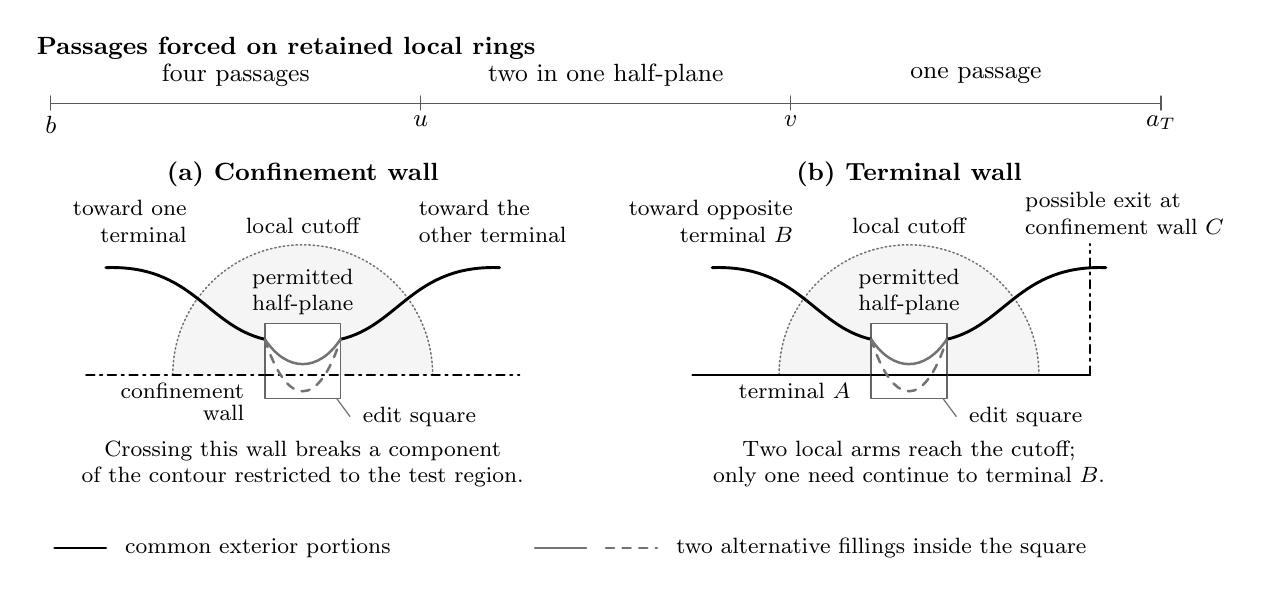
\begin{tikzpicture}[x=1cm,y=1cm,line cap=round,line join=round,
  every node/.style={font=\small},
  common/.style={black,line width=1.05pt},
  fillone/.style={black!55,line width=.9pt},
  filltwo/.style={black!55,line width=.9pt,dashed},
  cutoff/.style={black!55,line width=.55pt,densely dotted},
  confinement/.style={black,line width=.8pt,dash dot},
  terminal/.style={black,line width=.8pt}]

 \node[anchor=west,font=\small\bfseries] at (.15,6.6)
   {Passages forced on retained local rings};
 \draw[black!65] (.45,5.9)--(14.55,5.9);
 \foreach \x/\lab in {.45/b,5.15/u,9.85/v,14.55/a_T}{
   \draw[black!65] (\x,5.81)--(\x,5.99);
   \node[below,inner sep=2pt] at (\x,5.81) {$\lab$};
 }
 \node[align=center] at (2.8,6.25) {four passages};
 \node[align=center] at (7.5,6.25) {two in one half-plane};
 \node[align=center] at (12.2,6.25) {one passage};

 \begin{scope}[shift={(3.65,2.45)}]
  \node[font=\small\bfseries] at (0,2.55) {(a) Confinement wall};
  \fill[black!4] (-1.65,0) arc[start angle=180,end angle=0,radius=1.65]--cycle;
  \draw[cutoff] (-1.65,0) arc[start angle=180,end angle=0,radius=1.65];
  \node[font=\footnotesize] at (0,1.89) {local cutoff};
  \node[font=\footnotesize,align=center] at (0,1.05)
    {permitted\\half-plane};
  \draw[confinement] (-2.75,0)--(2.75,0);
  \node[anchor=east,font=\footnotesize] at (-.62,-.20) {confinement};
  \node[anchor=east,font=\footnotesize] at (-.62,-.48) {wall};
  \fill[white] (-.48,-.30) rectangle (.48,.65);
  \draw[black!60,line width=.55pt] (-.48,-.30) rectangle (.48,.65);
  \draw[confinement] (-.48,0)--(.48,0);
  \draw[common] (-2.5,1.36) .. controls (-1.4,1.4) and (-1.22,.62) .. (-.48,.45);
  \draw[common] (.48,.45) .. controls (1.22,.62) and (1.4,1.4) .. (2.5,1.36);
  \draw[fillone] (-.48,.45) .. controls (-.20,.03) and (.20,.03) .. (.48,.45);
  \draw[filltwo] (-.48,.45) .. controls (-.20,-.43) and (.20,-.43) .. (.48,.45);
  \node[font=\footnotesize,anchor=east,align=right] at (-1.35,1.95)
    {toward one\\terminal};
  \node[font=\footnotesize,anchor=west,align=left] at (1.35,1.95)
    {toward the\\other terminal};
  \draw[black!55,line width=.45pt] (.60,-.53)--(.43,-.30);
  \node[font=\footnotesize,anchor=west] at (.64,-.53) {edit square};
  \node[font=\footnotesize,align=center,text width=6.6cm] at (0,-1.13)
    {Crossing this wall breaks a component\\of the contour restricted to the test region.};
 \end{scope}

 \begin{scope}[shift={(11.35,2.45)}]
  \node[font=\small\bfseries] at (0,2.55) {(b) Terminal wall};
  \fill[black!4] (-1.65,0) arc[start angle=180,end angle=0,radius=1.65]--cycle;
  \draw[cutoff] (-1.65,0) arc[start angle=180,end angle=0,radius=1.65];
  \node[font=\footnotesize] at (0,1.89) {local cutoff};
  \node[font=\footnotesize,align=center] at (0,1.05)
    {permitted\\half-plane};
  \draw[terminal] (-2.75,0)--(2.30,0);
  \draw[confinement] (2.30,0)--(2.30,1.66);
  \node[anchor=east,font=\footnotesize] at (-.62,-.20) {terminal $A$};
  \fill[white] (-.48,-.30) rectangle (.48,.65);
  \draw[black!60,line width=.55pt] (-.48,-.30) rectangle (.48,.65);
  \draw[terminal] (-.48,0)--(.48,0);
  \draw[common] (-2.5,1.36) .. controls (-1.4,1.4) and (-1.22,.62) .. (-.48,.45);
  \draw[common] (.48,.45) .. controls (1.22,.62) and (1.4,1.4) .. (2.50,1.36);
  \draw[fillone] (-.48,.45) .. controls (-.20,.03) and (.20,.03) .. (.48,.45);
  \draw[filltwo] (-.48,.45) .. controls (-.20,-.43) and (.20,-.43) .. (.48,.45);
  \node[font=\footnotesize,anchor=east,align=right] at (-1.35,1.95)
    {toward opposite\\terminal $B$};
  \node[font=\footnotesize,anchor=west,align=left] at (1.35,2.05)
    {possible exit at\\confinement wall $C$};
  \draw[black!55,line width=.45pt] (.60,-.53)--(.43,-.30);
  \node[font=\footnotesize,anchor=west] at (.64,-.53) {edit square};
  \node[font=\footnotesize,align=center,text width=6.6cm] at (0,-1.13)
    {Two local arms reach the cutoff;\\only one need continue to terminal $B$.};
 \end{scope}

 \draw[common] (.5,.25)--(1.15,.25);
 \node[anchor=west,font=\footnotesize] at (1.27,.25) {common exterior portions};
 \draw[fillone] (6.6,.25)--(7.25,.25);
 \draw[filltwo] (7.5,.25)--(8.15,.25);
 \node[anchor=west,font=\footnotesize] at (8.27,.25) {two alternative fillings inside the square};
\end{tikzpicture}

\caption{Local geometry in Lemma~\ref{lem:stability-pivotal}.
The scale strip records the four-, two-, and one-passage regimes;
intervals may be empty, and rings near their endpoints are omitted
as in the lemma. Passages are counted by disjoint parameter intervals
and may lie on a single contour. The panels show the intermediate regime, with
the local cutoff below the next vertex and the other terminal.
Black contour portions agree outside the edit square; the two gray
fillings are alternatives. Crossing a confinement wall ends a
component restricted to the permitted region, whereas crossing a
terminal wall creates a terminal hit. In (b), one local arm may
later exit at the confinement wall~$C$, so the two local arms need
not form two full $A$--$B$ passages. The semicircular cutoffs are
schematic; the ring checks use the fixed crops and recenterings
specified in the lemma.}
\label{fig:pivotal-walls}
\end{figure}

\begin{proof}
Choose $a_T$ smaller than the separation of distinct nonincident
sides, the lengths of all sides, and the distances between the
disjoint terminal sets, with additional fixed reductions depending
on the finitely many vertex angles.  Then a ball below this scale
meets no test wall, just one straight wall, or walls incident to
one nearby vertex.  This choice is essential for a thin polygon:
distance to a vertex alone need not exclude a second, nonincident
side.  Capping at $a_T$ removes that difficulty.  Enlargement and
recentering cost only fixed factors for this test.

First work in a neighborhood meeting no test wall.  Cut the common
exterior contours at their intersections with the enlarged edit
square, making an arbitrarily small displacement of the cut to
avoid vertices.  Follow every exterior end to its first return to
the square or to the local outer cutoff.  An exterior connection
which reaches that cutoff supplies two long ends; short returns
can be contracted for this argument.  The number of long ends
is even.  If it is zero, the edit is screened within the cutoff.
If it is two, the interior filling, together with the short
exterior returns, must connect these same two ends in either
configuration.  It can add small closed curves but cannot change
their through connection or the two side colors seen outside the
cutoff.  Since there is no terminal in this neighborhood, these
small curves cannot create a terminal visit.  A changed passage
count therefore requires at least four long contour portions.
This argument is about cut parameter intervals, and allows all
four portions to come from one loop.

More explicitly, the filling together with short exterior returns
is a degree-two network whose only free ends are the long ends.
With two such ends it has one connecting path and terminal-free
cycles.  Restrict each resulting contour to the permitted test region,
breaking its parameter interval wherever it exits that region.  On each
remaining component record the successive inner and outer terminal
visits in parameter order, cyclically on a closed component, collapsing
consecutive visits of the same type.  The maximal
number of disjoint passages is the number of changes of terminal type
within these components.  A confinement-wall exit ends a component;
visits on opposite sides of such an exit are not paired.  Replacing
the terminal-free connecting path in the present wall-free neighborhood
preserves these sequences and their component endpoints.  This also
covers repeated visits by one contour and small terminal-free loops.

For a color-crossing test the same conclusion also follows by
juxtaposing a successful path and the blocking path of the
opposite color in the configuration where the test fails.  The
triangulation gives the exact crossing--blocking alternative.
Both paths must meet the edit square.  Outside it they supply
four alternating color continuations, whose intervening contours
give four long portions.  Cutting a band along a radial path
gives the identical argument for a circuit and its radial
blocker.

Next suppose that only one straight wall is present.  There are
two different wall roles for passage tests.  At a confinement
wall, a passage disrupted by the edit has a part on either side
of the disrupted portion leading back to the local cutoff in
the permitted half-plane; its terminal walls lie beyond that
cutoff.  These are the two required portions.  At a terminal
wall, stop every passage at its first terminal hit.  A portion
which hits this terminal before entering the edit neighborhood
is unchanged.  Among the remaining portions arriving from the
opposite terminal, a terminal hit can disappear only if the new
filling pairs its long end with another long end on the permitted
side.  Pairing with an end on the other side still crosses the
terminal wall and preserves a hit.  If there is only one long end
on the permitted side, neither pairing can remove the hit.
Consequently a changed terminal visit supplies two long portions
in the permitted half-plane.  A
hairpin tip moved across a terminal is covered by this case:
its two local arms supply the required half-plane portions.
In a confined test only one arm may continue all the way to the
opposite terminal, so the passage count need not change by two.

For a crossing and its blocker, at most the color arm directed
towards this single wall can terminate before the local cutoff.
The other three occur in alternating order on the permitted
side.  The two transitions between them give two disjoint
contour portions in that half-plane.  The circuit argument is
the same after the radial cut.  In each case start the
half-plane rings at a fixed multiple of the distance to the
wall and stop before the next vertex scale; the contours in
question stay on one consistent permitted side.  If the test
permits either side, taking the union of the two checks costs
at most a factor two per retained ring.

Above the vertex scale we retain only one contour portion.
For a crossing and blocker, two adjacent incident walls can
terminate two of the color continuations, but a transition
between the remaining colors persists towards the separated
terminal.  For a passage test, an affected passage still has
a portion towards its other terminal, at distance at least
$a_T$.  Equivalently, if no contour exits the local cutoff,
every change is confined to components which cannot connect
the separated terminal sets or alter a separating circuit.
Thus a pivotal change forces one passage up to $a_T$.

At every step the portions are cropped at the appropriate
first or last hits.  No positive-length interval is used
twice, even when a contour returns repeatedly to a wall.
The fixed-factor omissions accommodate the chosen cuts,
recentering, and the transition between the three geometric
regimes.  An $O(\delta)$ displacement of a wall is absorbed
by increasing the starting square and, for the half-plane
checks, translating its line outwards by $O(\delta)$.
\end{proof}

\subsection{A half-plane estimate under bulk conditions}

The pivotal-square lemma requires a bound $o(r/R)$ for two passages
constrained to one side of a bulk line.  We obtain it by counting
macroscopic subarcs, bounding the area of their near-support contacts,
and then separating off a four-passage alternative.
Propositions~\ref{prop:pure-four-passages} and~\ref{prop:pure-rsw}
give, for some $c>0$,
\begin{equation}
 \limsup_{\delta\downarrow0}\P_0(F_4(z,\theta;r,R))
       \leq C(r/R)^{2+c},
 \qquad
 \limsup_{\delta\downarrow0}\P_0(F_1(z,\theta;r,R))
       \leq C(r/R)^c.
 \label{eq:stability-pure-41}
\end{equation}
The ratios are fixed before the mesh limit.  Buffered comparisons
transfer these statements between the plane, a larger disk with plus
boundary, and bulk torus charts, with fixed multiplicative constants.
We next supply the estimate between them.  It concerns a geometric
half-plane inside a bulk chart, not a model with boundary conditions on
the straight line.

\begin{lemma}[Integrable numbers of macroscopic subarcs]
\label{lem:stability-counts}
Fix a compact region $K$ and a length $a>0$, in a bulk chart containing
a fixed $20a$-neighborhood of $K$.  There is a random finite list
$\mathcal L_\delta$ of compact contour parameter-subarcs, chosen without
reference to a test center or direction, with
$\sup_\delta\E|\mathcal L_\delta|<\infty$ for sufficiently fine meshes.
The list covers the following visits, with their contour multiplicities.
If a contour visits $x\in K$ and reaches distance $10a$ from $x$ in
both parameter directions, a member of the list contains that visit and
lies between the first such distant visit in each direction.  Subarcs
are retained only in a fixed enlargement of $K$.  The same assertion
holds for the limiting complete loop collection, with a list of finite
expected cardinality.  Fixed enlargements of the chart and fixed crops
of the excursion lengths only change the bound.
\end{lemma}

\begin{proof}
First consider a rectangle of fixed shape, with an unexamined buffer
around it.  Contour crosscuts between its horizontal sides, confined
between two vertical sides, are linearly ordered from left to right.
After cropping their ends, each crosscut has two colored side routes.
One obtains these routes by following the open spin regions next to
the interpolated contour and then following vertices in the
triangulation.  The two routes associated with one crosscut have
opposite signs.  Reading the routes in their planar order and retaining
successive sign changes produces an alternating list whose length is
at least a fixed fraction of the number of crosscuts.  Opposite signs
cannot meet.  Routes of the same sign separated by an opposite route
are disjoint as crossings.  The fixed end crop and side margins absorb
the interpolation distance.  Thus it suffices to bound the number of
ordered alternating spin crossings of a fixed rectangle.

Explore the leftmost crossing of a prescribed sign, if one exists.
The exploration examines only the sites on its left and the crossing
itself.  For example, reveal the vertices reachable from the examining
side before a crossing of that sign blocks the exploration; their
outer envelope gives the same leftmost path.  An alternative path
lying farther left somewhere is detectable on this examined side by
splicing at its first and last common vertices.  Consequently the
transcript leaves the spins to the right with the ordinary Ising
conditional law, and the only newly exposed spins facing that region
on the separating path have the prescribed sign.  Repeat for the
opposite sign in the remaining right region.  Previously examined
sites lie behind the most recent spanning path.

There is a uniform probability $c_0>0$, conditional on each successful
transcript, that no further opposite crossing can occur.  We construct
the blocking event in a deterministic rectangle, rather than asking RSW
for a crossing ending on the random exposed path.  For one fixed choice of proportions, take the counting slab to be
$[-1,1]\times[-2,2]$, and let $\Gamma$ be the exposed simple
color-$s$ crossing from its bottom to its top.  Use the central rectangle
$[-2,2]\times[-1,1]$ for a horizontal test, with end gates on
$x=-2$ and $x=2$, and surround it by the larger rectangle
$[-4,4]\times[-3/2,3/2]$.  Fixed changes of these proportions cover
the original rectangle shapes.

In the larger rectangle, fill the side to the left of $\Gamma$ by
color $s$, leave its right side free, and put color $-s$ on the outer
boundary.  The side is determined by the bottom-to-top crosscut in the
counting slab; its restriction to the central levels suffices, even
when it has bulges or crosses a horizontal level several times.
Nearest-neighbor conditional independence makes the filled left side
invisible from the right except through the color-$s$ path.  All
earlier revealed sites are screened by that path.  No sites to the
right of the counting slab have been examined, so the lateral extension
retains a free region past the right gate.  Thus, for increasing tests
when $s=+$, the actual remaining law dominates this right-side law;
putting the outer pins at minus only lowers it.  For $s=-$ the order
is reversed.

The filled comparison law in turn dominates, in the color-$s$ order,
the ordinary law in the same larger rectangle with all boundary spins
$-s$ and no interior pins.  In this last, deterministic law, a
color-$s$ horizontal crossing of the central test has probability at
least $c_0$ by Proposition~\ref{prop:pure-rsw}; its gates and test
collars are a positive distance from the outer pins.  Such a crossing
must meet $\Gamma$, since its gates lie on opposite sides of the
counting slab.  Its portion after the last meeting with $\Gamma$
connects the exposed path to the right gate.  It therefore blocks
another color-$-s$ vertical crossing confined to the slab.  This
suffix uses only the unexplored side, so the two monotone comparisons
prove the asserted conditional stopping probability.  The central
vertical crop leaves clearance from the endpoints of $\Gamma$;
lattice rounding is absorbed by the fixed margins.

The chance of continuing the alternating exploration after $m$
successful crossings is therefore at most $(1-c_0)^{m-1}$, with a
factor two for the initial color.  This gives uniformly bounded
moments of all orders for the number of contour crosscuts in a fixed
cropped rectangle.

Cover a fixed enlargement of $K$ by finitely many squares of diameter
much smaller than $a$.  Every departure by distance $a$ from one such
square contains a passage through one of finitely many buffered
rectangles; choose the first side through which an appropriate
enlargement is left.  Disjoint parameter intervals yield distinct
passages in this finite collection.  Their total number thus has
bounded expectation, indeed bounded moments.

Cut the contours at the boundary of an enlarged chart containing the
$20a$-neighborhood of $K$, and retain only components that meet $K$
and have diameter at least $10a$.
Subdivide each such parameter interval successively when its distance
from the last subdivision point first reaches $a$.  For a closed
component choose a root without reference to the later center or
direction and subdivide cyclically.  Retain every union of five consecutive
subdivision intervals whose middle interval meets $K$.  The interval
containing a qualifying visit is therefore the middle of one listed
union.  That union lies within distance less than $10a$ of the visit, after an absolute reduction of the
subdivision distance if needed.  It therefore lies between the two
distant visits in the statement.  The buffer from $K$ to the cutting
boundary ensures that these intervals exist on both sides of every
qualifying visit.  Endpoint remainders and cyclic intervals through a
root are included.  The rectangle count bounds the number of retained
intervals, including separate traversals of the same geometric region.
This constructs the required list without subdividing any part of a
contour far from the fixed chart.

Complete-resolution convergence from Theorem~\ref{thm:pure-cle},
with slightly relaxed rectangles, preserves every fixed finite
collection of these macroscopic passages.  Fatou's lemma transfers
the expectation bound to the limit.  Alternatively perform the same
successive subdivision on the limiting loops: uniform continuity
makes the list finite on each loop, and the relaxed passage counts
bound its expected length.  The construction lists no microscopic
loops unrelated to the excursions under consideration.
\end{proof}

\begin{lemma}[Area of near-support contacts]
\label{lem:stability-tangency}
Fix a bulk region and a positive excursion length.  For the pure
contours at mesh $\delta$, let $G_K(z,\theta,u)$ be the event that a contour subarc
comes within $C u$ of $z$, travels the fixed excursion length on both
sides of this visit, and throughout those two portions stays above
the line of direction $\theta$ through $z$ lowered by $CKu$.
For each fixed $K$,
\begin{equation}
 \limsup_{\delta\downarrow0}\P_0(G_K(z,\theta,u))=o_K(u),
 \label{eq:stability-tangency}
\end{equation}
as $u\downarrow0$ with $K$ fixed, uniformly over centers and directions
in a smaller bulk chart. Fixed crops or fixed changes of the constants
have the same conclusion.
\end{lemma}

\begin{proof}
Use a larger round disk with plus boundary as a reference and average
the center over the lattice translates of a small disk in its interior.
Translation invariance of the plane law and pure buffered density
comparison bound the plane probability at a specified center by
a constant times this averaged reference probability.  Off-lattice
centers are covered by an $O(\delta)$ relaxation of the distances.
This step uses only lattice translations.  Complete loop convergence
with relaxed distances then bounds its upper limit by the analogous
continuum event averaged over area.  Indeed every witnessing subarc
has a fixed positive diameter, so it belongs to the macroscopic part
of the loop ensemble; subsequential uniform parametrized convergence
preserves its closed near-visit and half-plane conditions after the
relaxation.  The reference disk and the
averaging disk are rotationally invariant.  We may therefore average
also over the direction in this continuum bound.  For directions or
centers varying with the mesh, take convergent subsequences and relax
the geometric inequalities before applying loop convergence.  This
gives the same uniform bound and does not assert rotational
invariance of the lattice.

Use Lemma~\ref{lem:stability-counts} with a subdivision length smaller
than one tenth of the fixed excursion length.  If the event occurs,
one member $C$ of its list contains the near visit and lies entirely
between the distant visits.  This list is independent of $z$ and
$\theta$.  Write $n_\theta$ and $t_\theta$ for the upward normal and
the unit tangent to the line, and put
\[
 m_C(\theta)=\min_{w\in C}n_\theta\cdot w,
 \quad
 C_{\theta,h}=\{w\in C:n_\theta\cdot w\leq m_C(\theta)+h\}.
\]
For almost every $\theta$ the support line of the compact convex hull
of $C$ has a unique contact point.  One elementary justification is
to use the support function of that convex hull: it is Lipschitz
on the circle and differentiable almost everywhere, and at a
differentiability direction the two extreme tangent coordinates of
the supporting face coincide.  Compactness then gives
\begin{equation}
 \operatorname{diam}\{t_\theta\cdot w:w\in C_{\theta,h}\}
       \longrightarrow0\qquad(h\downarrow0)
 \label{eq:stability-support-width}
\end{equation}
at each such direction.

If $C$ supplies a near visit, its height above its minimum at that
visit is at most $C_Ku$.  The normal coordinate of $z$ lies in an
interval of length $C_Ku$ about $m_C(\theta)$, and its tangent
coordinate lies within $Cu$ of the projection of $C_{\theta,C_Ku}$.
The area of the possible centers is therefore bounded by
\[
 C_Ku\left(\operatorname{diam}
          \{t_\theta\cdot w:w\in C_{\theta,C_Ku}\}+Cu\right).
\]
By \eqref{eq:stability-support-width} this is $o_K(u)$ for almost
every direction and is at most $C_Ku$ times a fixed chart diameter.
The expected number of arcs in the list is finite.  Dominated
convergence first over directions and then over that list proves
the averaged $o_K(u)$ bound.  The preceding buffered comparison and
rotational averaging yield \eqref{eq:stability-tangency}.
\end{proof}

\begin{proposition}[Two bulk passages confined to a half-plane]
\label{prop:pure-half-plane}
For the events in \eqref{eq:stability-checks}, in any buffered pure
bulk chart,
\begin{equation}
 \limsup_{\delta\downarrow0}\P_0(H_2(z,\theta;r,R))=o(r/R)
 \quad\text{as }r/R\downarrow0.
 \label{eq:stability-halfplane}
\end{equation}
The ratio is fixed before taking the mesh limit.  The assertion is
uniform in translations and rotations of the fixed geometry, and
continues to hold with fixed proportional crops.
\end{proposition}

\begin{proof}
Normalize $R=1$ and write $u=r/R$.  Select two confined passages.
If there are fewer than four unconstrained passages from radius
$u$ to radius $Ku$, they belong to the same loop and their inner
ends are joined inside radius $O(Ku)$.  To verify the statement
including multiplicities, first suppose that the selected passages
belong to different loops.  The complementary arc on each loop
supplies a second passage to $Ku$, giving four in total.  On a
single loop the two complementary arcs either both join an inner
end to an outer end, again giving four, or join inner to inner and
outer to outer.  In the latter case an excursion of the inner
connecting arc to $Ku$ supplies two further passages.  These may
share their outer hit, as allowed by our convention, and have
disjoint interiors.  Thus that excursion is excluded.

Concatenate the two confined passages and their inner connecting
arc.  This subarc has a near visit to $z$ and goes a fixed positive
distance on both sides, all above the original line lowered by
$CKu$.  Its probability is $o_K(u)$ by
Lemma~\ref{lem:stability-tangency}.  In the complementary case there
are four passages from $u$ to $Ku$, and the original confined
passages still give two confined passages from $C_0Ku$ to $1$.
Here $C_0$ is a fixed buffer constant.  Condition on the spins
outside radius $C_0Ku$.  Pure buffered comparison bounds the
conditional four-passage probability by $CK^{-2-c}$, uniformly in
those outside spins, by \eqref{eq:stability-pure-41}.

Let $p(u)$ be the mesh upper limit of the plane confined-passage
probability, with the uniform translation and direction convention
just described.  We have proved, for every sufficiently large fixed
$K$ and all sufficiently small $u$,
\begin{equation}
 p(u)\leq o_K(u)+CK^{-2-c}p(C_0Ku).
 \label{eq:stability-half-recursion}
\end{equation}
All constants associated with buffers and relaxed squares are fixed
before $K$ is enlarged.  Square and Euclidean radii differ by fixed
factors and give the same recursion after changing $C_0$.

For completeness, put $q(u)=p(u)/u$, $d=C_0K$, and
$\vartheta=CC_0K^{-1-c}$.  Fix $K$ so large that $\vartheta<1$.
Then $q(u)\leq e_K(u)+\vartheta q(du)$, where $e_K(u)\to0$.
Iterate until $d^mu$ first reaches a fixed small interval bounded
away from zero.  The terminal value is bounded because $p\leq1$,
and
\[
 q(u)\leq\sum_{j=0}^{m-1}\vartheta^j e_K(d^ju)
                 +\vartheta^m q(d^mu).
\]
This first gives boundedness of $q$ near zero.  Splitting the sum
at a fixed index, letting $u\downarrow0$, and then sending that
index to infinity gives $q(u)\to0$.  This proves the plane
assertion.  A final fixed buffered density comparison proves the
same assertion in the other pure bulk charts.
\end{proof}

The three pure probabilities now decay more strongly than their
respective location counts.  We need their consequence at one large
fixed annulus ratio, together with a product rule.  Neither step will
refer to the law of a configuration after it has been edited.

\subsection{Conditional ring products with independent marks}

At a given stage allow only marks of radius at most $b$.  A check on
an annulus is determined by the original spins in that annulus with
an $O(\delta)$ margin, and by the mark variables whose squares meet
this support.  It does not require the assigned spins outside this
support.  Denote its support by $A_j$ and this finite set of mark
indices by $\mathcal J_j$.

\begin{lemma}[Ring product bound]
\label{lem:stability-products}
There is a fixed constant $D$ with the following property.  Take
annular checks of the types \eqref{eq:stability-checks}, whose inner
radii exceed $C b$, and whose enlarged neighborhoods and
proportional inner and outer collars are disjoint.  More precisely,
after absorbing rotations and lattice margins, each check has a
collar $W_j$ of the form
\[
 S_{2R_j}(z_j,\theta_j)\setminus
       S_{r_j/2}(z_j,\theta_j),
\]
the other check supports lie outside $W_j$, and the sets
$\mathcal J_j$ are disjoint.  All collars lie in bulk torus charts.
For arbitrary independent mark probabilities at or below this
cutoff,
\begin{equation}
 \P\left(\bigcap_{j=1}^m T_j^+\right)
       \leq\prod_{j=1}^m D\P(T_j^+).
 \label{eq:stability-product}
\end{equation}
The constant $D$ depends on the fixed collar proportions and is
independent of the annular aspect ratios and the mark probabilities.
\end{lemma}

\begin{proof}
Condition on the original pure spins outside $W_j$ and on all marks
outside $\mathcal J_j$.  For each fixed value of the remaining
local marks, $T_j^+$ is simply an event of the pure spins on $A_j$.
Corollary~\ref{cor:pure-annular} gives the pointwise density bound
\begin{equation}
 \frac{d\mu_{0,N}(\sigma_{A_j}\mid\sigma_{W_j^c})}
      {d\mu_{0,N}(\sigma_{A_j})}\leq D.
 \label{eq:stability-ring-density}
\end{equation}
For clarity, the two parts of this comparison have fixed aspect:
the outer data are separated from $A_j$ by the collar outside
$S_{R_j}$, and the inner data by the collar inside $S_{r_j}$.
For the second comparison interchange the terminal sets in the
symmetric density-odds bound and regard the already fixed outer
data as common pins.  The two losses are independent of $R_j/r_j$.
No pins occur in the intervening free collars.

For rotated squares this comparison uses a fixed patch cover, as in
\cite[Corollary~2.6]{OpenAIStatic2026}, without rotating the lattice. Write $S_t=z+e^{i\theta}[-t,t]^2$.
Partition $A=S_R\setminus S_r$ into a bounded number of sets, each
contained in an axis-aligned square of radius $cR$, with $c>0$ fixed
and small. Each patch is separated from the changed data outside
$S_{2R}$ by a distance comparable to $R$, uniformly in $\theta$.
Factor the probability of the configuration on $A$ into successive
patch conditionals. Earlier patches and all inner data are common
pins, allowed by Proposition~\ref{prop:pure-buffered}, so the bounded
product costs a fixed factor. To change the inner data, partition
$S_{r/2}$ into a bounded number of patches of diameter $cr$ and change
them one at a time. Each is separated from the whole observed annulus
by distance comparable to $r$. Terminal symmetry gives the same bound,
with the remaining inner patches and the outer data common. These
two finite products are uniform in $R/r$ and $\theta$. Finally mix
the reference exterior data to obtain
\eqref{eq:stability-ring-density}. Fixed positive patch clearances
absorb lattice rounding.

The marks in $\mathcal J_j$ are independent of the conditioning
and of the original spins.  Integrating the pointwise bound over
their unchanged distribution gives
\[
 \P(T_j^+\mid\sigma_{W_j^c},M_{\mathcal J_j^c})
       \leq D\P(T_j^+).
\]
All other $T_i^+$ are measurable with respect to this conditioning.
Remove the factors one at a time to obtain
\eqref{eq:stability-product}.  This proof uses conditional laws
of $\sigma^0$ only.  In particular, it neither defines nor assumes
a conditional mixing estimate for an edited spin law.
\end{proof}

Choose a large fixed gap factor $G$.  In a range of available scales
retain rings of ratio $A$ whose successive inner radii have ratio
$GA$.  For $G$ large enough their collars and mark-index
neighborhoods satisfy Lemma~\ref{lem:stability-products}, including
the harmless recenterings of Lemma~\ref{lem:stability-pivotal}.
Fix also a monitoring constant $C_{\rm mon}$ larger than the
minimum-radius constant in Lemma~\ref{lem:stability-products}, enlarged
to allow the fixed crops and recenterings.  Around an inserted square
of radius $b$, begin each retained ring only when its inner radius
is at least $C_{\rm mon}b$.  Removing the preceding rings costs a
bounded number of rings, absorbed in the pivotal bound below.
Thus every retained check is among the checks monitored at that
activation stage; this is the scale closure used in the bootstrap.
First choose these constants and the density constant $D$.  Then choose $A$
large.  By \eqref{eq:stability-pure-41} and
Proposition~\ref{prop:pure-half-plane}, the three pure probabilities
at ratio $A$ can be made small enough that there are numbers
\begin{equation}
 p_4>2,\qquad p_h>1,\qquad p_1>0,
 \label{eq:stability-exponents}
\end{equation}
pure probability bounds $q_4,q_h,q_1$, and positive tolerances
$\tau_4,\tau_h,\tau_1$ such that
\begin{equation}
 D(q_i+\tau_i)<(GA)^{-p_i},\qquad i\in\{4,h,1\}.
 \label{eq:stability-slack}
\end{equation}
Increase $D$ first to include the possible two choices of
half-plane and any other fixed union of cropped checks.
The assertion for $h$ uses $q_h=o(A^{-1})$: after $G,D$ are fixed,
one can choose $A$ with $Dq_h<(GA)^{-1}$ with strict slack, and
then choose $p_h>1$ sufficiently close to one.  It does not require
a previously known half-plane power law.  The assertion for $4$
uses the strict exponent above two.  The assertion for $1$ uses
any positive one-passage exponent.

All these choices precede $s_0$.  At this fixed ratio, increase
$s_0$ so that the pure finite-mesh bounds $q_i$ hold uniformly
for every translated and rotated check with inner lattice radius
at least a fixed multiple of $Ls_0$, in the stated torus charts.
Such a threshold follows from the mesh-first pure estimates and
buffered comparison.  If uniformity in the frame failed, take
convergent directions and normalized offsets and use slightly
relaxed radii; their fixed margins give the same estimate.
This is a choice for three fixed shapes, rather than a uniform
claim over an increasing family of final polygonal tests.

Suppose for the moment that, with marks of radii at most $b$,
the probabilities of all needed possibility checks are at most
$q_i+\tau_i$.  Pack the retained rings in the three ranges of
Lemma~\ref{lem:stability-pivotal}.  Omitting only the bounded
number of transition rings, \eqref{eq:stability-product} and
\eqref{eq:stability-slack} give the following bound for the
possibility of a pivotal insertion of a square of radius $b$:
\begin{equation}
 C_T\left(\frac b u\right)^{p_4}
     \left(\frac u v\right)^{p_h}
     \left(\frac v{a_T}\right)^{p_1},
 \qquad b\leq u\leq v\leq a_T.
 \label{eq:stability-pivotal-probability}
\end{equation}
This probability does not include the mark of the inserted square.
If its addition first permits a different test value, choose a
witnessing assignment afterwards and revert the new square to
the old values, retaining all other assignments.  The two
configurations agree outside that square.  The required checks
outside it are therefore possible using the previous marks.
They are exactly the events to which the product bound applies.

\subsection{The area sum and the finite-size bootstrap}

\begin{lemma}[Counting potential insertion centers]
\label{lem:stability-area}
Assume the possibility bounds just used.  For a fixed polygonal
test $T$, the total contribution to its change probability from
all marks of level $k$ is at most
\begin{equation}
 C_T\epsilon 2^{-k}
       \min\{1,(\delta b_k^{\mathrm{lat}}/a_T)^{c_*}\},
 \label{eq:stability-level-bound}
\end{equation}
for a fixed $c_*>0$.  The assertion also holds during any spatially
nonuniform partial activation of that level.  For the three
fixed annular shapes the constant is uniform in their scale,
position, and rotation.
\end{lemma}

\begin{proof}
Use physical lengths and rescale $a_T$ to one.  Write
$b=\delta b_k^{\mathrm{lat}}/a_T$, and similarly rescale $u,v$.
Discard centers whose edit square does not meet the finite spin
support of $T$: their insertion cannot affect the test.
For $b\leq1$, divide the insertion centers into dyadic classes
with truncated distances comparable to $u,v$, where
$b\leq u\leq v\leq1$.  The area of one such class is at most
$C_Tuv$.  Indeed, when $v<1$ the relevant portion of an edge
has length $O_T(v)$ near a vertex, and its $u$-neighborhood
has area $O_T(uv)$.  When $v$ is comparable to one, the total
finite edge length is $O_T(1)$.  Centers far from the edges
belong to the capped class $u=v=1$.  Lower truncation at $b$
allows the same estimate after enlarging by one lattice cell,
so there are at most $C_Tuv/\delta_T^2$ centers, where
$\delta_T=\delta/a_T$ is the rescaled mesh.

The marking probability is bounded by
$C_L\epsilon2^{-k}\delta_T^2/b^2$.  Multiplication by the
number of centers and \eqref{eq:stability-pivotal-probability}
gives exactly
\begin{align}
 &C_T\epsilon2^{-k}\frac{uv}{b^2}
          (b/u)^{p_4}(u/v)^{p_h}v^{p_1}\nonumber\\
 &\hspace{15mm}=
 C_T\epsilon2^{-k}
          (b/u)^{p_4-2}(u/v)^{p_h-1}v^{p_1}.
 \label{eq:stability-area-factor}
\end{align}
This equality is where both location-count thresholds enter.
Let
$m=\min\{p_4-2,p_h-1,p_1\}>0$.  The three base ratios in the
last line belong to $(0,1]$ and their product is $b$.  Every
term is therefore at most $C_T\epsilon2^{-k}b^m$.
There are $O_T((1+\log(1/b))^2)$ dyadic pairs.  Absorbing
this factor into $b^{m/2}$ proves
\eqref{eq:stability-level-bound}, with $c_*=m/2$.

If $b\geq1$, the centers whose squares can affect the test
occupy area at most $C_Tb^2$.  The crude bound one on
pivotality, combined with the marking probability, gives
$C_T\epsilon2^{-k}$.  The same crude count covers $b$ within
a fixed factor of one.  Omitted transition rings at smaller
scales have already been absorbed into $C_T$ in
\eqref{eq:stability-pivotal-probability}.
The computation uses only upper bounds on individual mark
probabilities; partial activation can therefore be arbitrary
in space.  For a fixed annular shape the geometric constants
scale with its inner radius and are independent of its
location or orientation.
\end{proof}

\begin{proposition}[Uniform bootstrap of the three checks]
\label{prop:stability-bootstrap}
There is $\epsilon_*>0$, chosen from the three fixed annular
shapes and the fixed constants of the mark law, such that the
following holds on every sufficiently fine finite torus.
Activate the independent marks in order of increasing radius.
At a stage with maximum permitted radius $b$, every check of
ratio $A$ with inner radius at least $C_{\rm mon}b$, and with its
prescribed bulk collars, satisfies
\begin{equation}
 \P(T_i^+)\leq q_i+\tau_i,
 \qquad i\in\{4,h,1\}.
 \label{eq:stability-bootstrapped}
\end{equation}
This remains true throughout continuous, possibly spatially
nonuniform activation of marks of the current radius.
\end{proposition}

\begin{proof}
There are finitely many mark variables on the torus.  Activate
one level at a time, increasing its Bernoulli parameters
continuously from zero to their prescribed values.  Conditional
on the pure spins, the expectation of an increasing event of
these marks is a polynomial in their parameters.  Differentiating
in a parameter gives the probability that this index is pivotal
when its own mark is omitted.  Integration is the usual
finite-product interpolation identity and requires no monotonicity
in the spins.  For any collection of checks, even a continuum
of geometric frames, these expectations are uniformly Lipschitz
in the finitely many parameters: the sum of their absolute
parameter changes bounds the change of every event probability.
Thus their supremum is continuous as well.

Before any marks are activated, the estimates hold with strict
slack, by the choice of $s_0$.  At each stage monitor only
checks with inner radius at least $C_{\rm mon}$ times the current radius.
When the cutoff increases, some checks leave this collection.
They are not needed again: the rings used for a later insertion
start at a larger fixed multiple of that insertion's radius.
Conversely, any check still monitored at a given stage has
been monitored throughout all earlier stages.

Suppose there were a first failure of
\eqref{eq:stability-bootstrapped}.  Up to that stage all ring
possibility estimates used to control an insertion satisfy
\eqref{eq:stability-bootstrapped}; by continuity the same weak
bounds hold at the candidate first failure.  Each pivotal
insertion for any monitored check therefore satisfies
\eqref{eq:stability-pivotal-probability}.  Apply
Lemma~\ref{lem:stability-area} to that check, summing all
previous levels and the activated fraction of the current
level.  Since these checks are translates, rotations, and
dilates of only three fixed shapes, their total probability
increase is at most
\[
 C_{\mathrm{boot}}\epsilon\sum_{k\geq0}2^{-k}
       \leq2C_{\mathrm{boot}}\epsilon.
\]
Choose $\epsilon_*$ so that this is less than
$\frac12\min_i\tau_i$.  The first failure cannot occur.
The same estimate, being uniform over the frames, rules out
a failure occurring only as a supremum.  This proves the
bootstrap on each finite torus, before taking any limit.

The order of the choices is now explicit: fix the collars
and gap factor, choose $A$ and the tolerances, enlarge $s_0$,
and then choose $\epsilon_*$.  The finitely many universal
shapes determine $C_{\mathrm{boot}}$.  No later polygonal
test enters this choice.  The enlargement of $s_0$ is made
before the critical trajectory of
Theorem~\ref{thm:critical-trajectory} is constructed.
\end{proof}

\subsection{Vanishing for every fixed family}

\begin{proof}[Proof of Theorem~\ref{thm:bulk-stability}]
Fix one of the tests $T$ in the statement.  During increasing
activation of the marks, apply the finite-product interpolation
identity to $D_T$.  Its initial value is zero.  If a new mark
first makes $D_T=1$, choose two permitted assignments with
different test values and revert the newly permitted square
in a witnessing assignment.  Before its addition all
assignments gave one value.  We obtain two configurations
which differ only inside that square and change the test.
Lemma~\ref{lem:stability-pivotal} applies, and its required
outside checks are possibility events using the older marks.
Proposition~\ref{prop:stability-bootstrap} controls these
checks whenever the insertion is smaller than the test.
For larger insertions use the crude overlapping-square count
in Lemma~\ref{lem:stability-area}.  We conclude that
\begin{equation}
 \P(D_T=1)\leq C_T\epsilon
       \sum_{k\geq0}2^{-k}
       \min\left\{1,
          \left(\frac{\delta(Ls_k+O(1))}{a_T}\right)^{c_*}\right\}.
 \label{eq:stability-final-sum}
\end{equation}
Absent torus levels can be set to zero; the displayed
infinite sum is a convenient upper bound.  For every fixed
$k$, its factor in braces tends to zero with $\delta$.
Every summand is dominated by $2^{-k}$, whose sum is finite.
Dominated convergence therefore proves $\P(D_T=1)\to0$.
Equivalently first make the level tail small, and then refine
the mesh for the finitely many remaining levels.  This
argument keeps $\epsilon$ fixed; it does not require a new
smallness condition depending on $C_T$.

A union bound proves \eqref{eq:stability-main} for the fixed
finite family.  Under Proposition~\ref{prop:edit-coupling},
the perturbed configuration belongs to
$\mathcal C(\sigma^0,M)$ except with probability $o(1)$.
On the complement of that exceptional event and all $D_T$,
the entire test vector agrees with the pure vector.  Its
total-variation distance from the pure test-vector law tends
to zero.  The joint positivity and four-passage conclusions
follow respectively from Proposition~\ref{prop:pure-rsw}
and Proposition~\ref{prop:pure-four-passages}.
\end{proof}

We record the precise quantifiers in the upper-bound consequence.
For every fixed buffered square annulus of radii $r,R$,
\begin{equation}
 \limsup_{\delta\downarrow0}\P_{\mathrm{pert}}(F_4(z,\theta;r,R))
 \leq
 \limsup_{\delta\downarrow0}\P_{0,N}(F_4(z,\theta;r,R))
 \leq C(r/R)^{2+c}.
 \label{eq:stability-perturbed-four}
\end{equation}
Only after this mesh limit do we send $r/R$ to zero.  In particular,
for a fixed compact chart and fixed $R$, cover the possible centers
by an $r$-grid, enlarge the inner squares by a fixed factor, and
reduce the outer radius from $R$ to $R/2$.
The finite union for each fixed $r$ has at most $C r^{-2}$ members.
Applying \eqref{eq:stability-perturbed-four} to that finite family
and then sending $r\downarrow0$ gives
\begin{equation}
 \lim_{r\downarrow0}\limsup_{\delta\downarrow0}
 \P_{\mathrm{pert}}\bigl(\text{some center in the compact chart has
 four passages from }r\text{ to }R\bigr)=0.
 \label{eq:stability-compact-bottlenecks}
\end{equation}
Thus the family grows only after its own mesh limit has been taken.
Later fixed-buffer density comparisons will transfer this statement
from torus charts to the interior of the specified finite domains.
